\section{三角函数与周期：用旋转描述重复变化}
\label{sec:02-Calculus/01-Functions-and-Precalculus/05}

一份服务请求量的日志，按小时聚合，画出来先做一条趋势线。趋势线抓住了整体缓慢上升的部分，可残差图上还剩着一道明显的形状：每天凌晨压到最低，傍晚拱到最高，一天一个来回，从不走样。

多项式帮不上忙。任何非常数多项式在 \(t\) 变大时要么冲上去要么掉下去，不会老老实实回到原处再来一遍。上一节的指数函数同样是一路朝一个方向走。要描述``重复''，需要一族天生就会绕圈的函数。

\subsection{周期是转满一圈的后果}

直角三角形只能定义锐角的正弦余弦，负角、超过一周的角、连续旋转都装不进去。单位圆一次性解决：从点 \((1,0)\) 出发逆时针转过 \(\theta\)，落点的横坐标记作 \(\cos\theta\)，纵坐标记作 \(\sin\theta\)。

这样一改，三角函数就不再是三角形的边长比，而是旋转的坐标读数。周期性也不需要另行规定——转过 \(2\pi\) 回到同一个点，坐标当然一模一样。勾股定理同时白送一条恒等式 \(\sin^2\theta+\cos^2\theta=1\)，它说的无非是那个点始终在半径为 \(1\) 的圆上。

\begin{center}
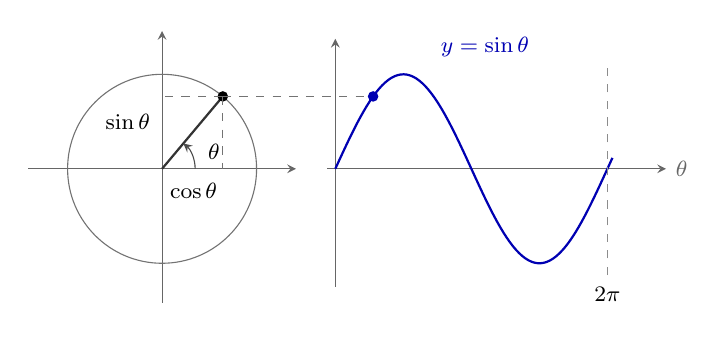
\begin{tikzpicture}[x=1cm,y=1cm,font=\small,>=stealth]
  \draw[->,black!60] (-1.7,0) -- (1.7,0);
  \draw[->,black!60] (0,-1.7) -- (0,1.75);
  \draw[black!55] (0,0) circle (1.2);
  \draw[black!80,thick] (0,0) -- (0.771,0.919);
  \fill (0.771,0.919) circle (1.9pt);
  \draw[black!55,dashed] (0.771,0.919) -- (0.771,0);
  \draw[black!55,dashed] (0.771,0.919) -- (0,0.919);
  \node[below,font=\footnotesize] at (0.40,-0.06) {\(\cos\theta\)};
  \node[left,font=\footnotesize] at (-0.03,0.60) {\(\sin\theta\)};
  \draw[->,black!70] (0.42,0) arc (0:50:0.42);
  \node[font=\footnotesize] at (0.66,0.22) {\(\theta\)};
  \draw[->,black!60] (2.1,0) -- (6.4,0) node[right,font=\footnotesize] {\(\theta\)};
  \draw[->,black!60] (2.2,-1.5) -- (2.2,1.65);
  \draw[blue!70!black,thick] plot[domain=0:6.4,samples=90] ({2.2+0.55*\x},{1.2*sin(\x r)});
  \draw[black!55,dashed] (0.771,0.919) -- (2.66,0.919);
  \fill[blue!70!black] (2.68,0.919) circle (1.9pt);
  \draw[black!45,dashed] (5.656,-1.35) -- (5.656,1.35);
  \node[below,font=\footnotesize] at (5.656,-1.38) {\(2\pi\)};
  \node[font=\footnotesize,blue!70!black] at (4.1,1.55) {\(y=\sin\theta\)};
\end{tikzpicture}

\emph{左边匀速转圈，把那一点的纵坐标随角度画出来，就是右边的正弦波。波形不是被规定成这样的，它是投影的结果；同理，周期等于 \(2\pi\) 也不是额外假设，而是``转一圈回到同一点''这句话的另一种说法。}
\end{center}

这个视角在后面会不断加码。旋转、复数的辐角、Fourier 分解里的基函数，用的都是这张图；把一维的重复看成二维旋转的投影，是贯穿信号处理与线性代数的一条主线。

\subsection{弧度不是换算习惯，是换了函数}

弧度定义为弧长除以半径，单位圆上转过角 \(\theta\) 对应的弧长恰好是 \(\theta\)。微积分默认弧度，理由不是好看，而是只有在弧度下才有

\[
\lim_{h\to0}\frac{\sin h}{h}=1,
\]

从而 \((\sin x)'=\cos x\) 干干净净，不带系数。若把变量换成度数，同一个符号 \(\sin\) 指的已经是另一个函数——它在 \(0\) 附近的上升速度是原来的 \(\pi/180\)，所有导数公式都要挂上这个因子。计算器或库函数的角度模式设错了，后果不是精度差一点，是整条链路在算别的东西。

\subsection{四个参数各管一件事}

周期现象的通用写法是

\[
y(t)=A\cos\bigl(\omega(t-t_0)\bigr)+D .
\]

\(D\) 定中线，也就是波动围绕的水平位置；\(|A|\) 定振幅，即离中线最远多少；\(\omega\) 定快慢，周期是 \(T=2\pi/|\omega|\)；\(t_0\) 定相位，也就是峰值出现在哪一刻。把式子写成 \(\omega(t-t_0)\) 而不是 \(\omega t+\varphi\) 是有讲究的：前者把峰值时刻直接摆在眼前，后者要靠 \(-\varphi/\omega\) 算一道。这里的符号坑和本章第二节的横向平移是同一个——括号里减去 \(t_0\)，波形往右挪 \(t_0\)。

开头那份日志就可以写成 \(20+5\cos\bigl(\tfrac{2\pi}{24}(t-15)\bigr)\) 这种形状：中线 \(20\)，振幅 \(5\)，周期 \(24\) 小时，峰值落在下午三点。真实数据当然不会严格是余弦，这个模型只保留了主日周期，剩下的部分交给别的项。

一个周期不够用时就叠加多个。年度数据里同时藏着周周期和年周期，加两组正余弦即可；Transformer 的位置编码走的是同一条路，几十个通道用几十个从快到慢的 \(\omega\)，把一个位置编号摊成一串有界的坐标，位置相差多少在每个尺度上都对应一次固定角度的旋转（见\hyperref[ch:127]{``注意力与序列：让内容决定从哪里读取信息''}）。直接把位置编号本身喂进网络会带来一个无界且随序列长度漂移的量，换成正余弦之后取值永远在 \([-1,1]\) 内，这是选择周期函数的实际理由之一。

\subsection{反三角函数必须先划一段}

正切定义为 \(\tan\theta=\sin\theta/\cos\theta\)，在 \(\cos\theta=0\) 处没有定义，周期是 \(\pi\) 而不是 \(2\pi\)。图像上那些竖直渐近线来自分母趋于零，不是函数在那里取到了``无穷大''这个值——渐近线是行为描述，不是函数值。

更要紧的是反向读取的问题。用本章第三节的水平线检验一量就知道，任何周期函数在整个实数轴上都不是单射，一条水平线会切中它无穷多次。所以反三角函数不可能直接存在，必须先把定义域砍到一段单调区间上，这段区间叫主值区间：

\[
\arcsin:[-1,1]\to[-\pi/2,\pi/2],
\qquad
\arccos:[-1,1]\to[0,\pi],
\qquad
\arctan:\R\to(-\pi/2,\pi/2).
\]

这是第三节处理 \(x^2\) 时那套办法的原样重演，只不过碰撞的数量从两个变成了无穷多个。让出的东西也一样：恒等式只在选定的那一段上成立。\(\arcsin(\sin x)\) 并不总等于 \(x\)，超出主值区间的角会被折回来，\(x=3\pi/4\) 时得到的是 \(\pi/4\)。凡是写反函数恒等式，就得连同它的论域一起写。

\subsection{这一章交出去的和留下的}

本章从头到尾只做了一件事：把``什么量依赖什么量''说清楚。函数是定义域、陪域与对应规则的三件套，图像是观察它的一扇窗；复合把简单函数串成流水线，可逆性回答这条流水线能不能倒放；指数刻画固定倍数的推进，三角函数刻画绕圈重复。这些是后面所有讨论的共用语言。

但这套语言目前还只能描述静止的对应关系。它说得出 \(f\) 在每一点取什么值，说不出 \(f\) 在某一点附近怎样变化；它区分得了连续的图像和裂开的图像，却还没有一句话能精确定义``裂开''。本章第一节末尾那道分段函数的裂口就卡在这里——左边飘向 \(1\)，右边停在 \(0\)，而``飘向''二字至今没有定义。\hyperref[ch:011]{``极限与连续：不必到达，也能控制趋势''}一章补上的正是这个词。
